\section{Related Work and Positioning}
\label{sec:related-work}

The previous two sections introduced the methods this work studies:
data augmentation and self-supervised representation learning. But
these are not the only approaches to data-efficient RL. Three other
families of methods have demonstrated strong results on Atari-100K:
world models, planning methods, and training efficiency
improvements. This section briefly surveys each family, then
positions the contribution of this work relative to the field. The
survey describes what each approach does and how it relates to our
work, not how it works internally -- the reader needs context, not
a second background chapter.

\subsection{World Models}
\label{subsec:world-models}

A world model learns to predict what happens next: given the
current state and action, predict the next state and reward. Once
learned, the model can generate imagined experience -- the agent
can simulate trajectories without interacting with the real
environment. This addresses data efficiency directly: if real
interactions are expensive, generate synthetic ones from the model.
SimPLe~\citep{kaiser2020model} demonstrated this approach on Atari
by learning a video prediction model from real frames, then
training the agent on a mixture of real and model-generated
rollouts. Pixel-level prediction is expensive, however, and model
errors compound over long imagined horizons, making the generated
frames increasingly unreliable.

\smallskip
Dreamer~\citep{hafner2020dream} and
DreamerV2~\citep{hafner2021mastering} address this limitation by
learning a world model in \emph{latent space}. The model predicts
future latent states rather than future pixels, and the policy is
trained entirely in the model's imagination. This is more efficient
than pixel prediction and represents a fundamentally different
paradigm: the agent's decision-making is model-based, while DQN
(even with SPR) remains model-free.

\smallskip
World models and SPR share a structural similarity: both learn to
predict future states. But they differ in what the predictions are
used for. World models use predictions to generate experience for
training or planning -- the model is a core component of the
agent's decision-making. SPR uses predictions only as a training
signal to shape the encoder's representations; the transition model
is discarded at test time. SPR is therefore simpler -- it does not
need accurate long-horizon predictions or reward prediction -- but
it cannot leverage model-generated data.

\subsection{Planning Methods}
\label{subsec:planning-methods}

Planning methods combine a learned model with tree search.
MuZero~\citep{schrittwieser2020mastering} learns a latent model
optimized end-to-end for planning: at test time, the agent runs
Monte Carlo tree search (MCTS) in latent space, simulating possible
action sequences, evaluating them with the learned model, and
selecting the best action.
EfficientZero~\citep{ye2021mastering} adapted MuZero for the
data-efficient regime by adding self-supervised consistency
regularization, achieving superhuman performance on several
Atari-100K games -- the strongest results on the benchmark at the
time of publication.

\smallskip
Planning methods and SPR both learn predictive models, but they
differ in how those models are used. Planning methods use the
model at test time for action selection: MCTS requires many forward
passes per decision. SPR uses the model only at training time; the
agent is model-free at test time, with the same computational cost
as vanilla DQN (one forward pass per action). This work does not
compare against planning methods -- they address data efficiency
through a fundamentally different paradigm.

\subsection{Training Efficiency}
\label{subsec:training-efficiency}

A third family of methods improves data efficiency not by learning
a model or adding auxiliary objectives, but by training the
existing agent more effectively.
BBF~\citep{schwarzer2023bigger} scales the encoder from the
five-layer Nature CNN to a substantially deeper architecture
(a residual network, or ResNet) and introduces periodic network
resets to combat \emph{plasticity loss} -- the phenomenon where
neural networks gradually lose the ability to learn new features as
training progresses. BBF also uses SPR as part of its training
objective, meaning its strong results include SPR's contribution on
top of the network scaling and training improvements.
SR-SPR~\citep{doro2023sampleefficient} extends SPR's prediction
target to include successor representation features, combining
temporal prediction with value-based prediction to push replay
ratios higher than previously possible.

\smallskip
These methods change how the agent trains; this work studies what
the representations learn. BBF's use of SPR means its results
cannot be attributed to SPR alone -- the same attribution problem
that motivates our study, at a different level. The two lines of
work are complementary: we isolate SPR's representation learning
contribution, while training efficiency work asks how to maximize
a fixed training budget.

\subsection{Positioning}
\label{subsec:positioning}

\Cref{fig:method-landscape} summarizes the landscape. Each family
addresses the limited-data problem through a different mechanism,
but none ask when representation learning works or what determines
whether the learned representations are useful.

\begin{figure}[htbp]
\centering
% Thesis-wide categorical color palette
% Usage: % Thesis-wide categorical color palette
% Usage: \input{figures/palette} in any figure file
%
% Muted primary colors -- print-friendly, visually distinct.
% Inspired by Cooper Union's red/blue primaries, softened for
% academic figures. Use palA-palC for data series in scatter
% plots, line charts, bar charts, etc.

\definecolor{palA}{HTML}{1F77B4}   % Tableau blue
\definecolor{palB}{HTML}{D62728}   % Tableau red
\definecolor{palC}{HTML}{2CA02C}   % Tableau green
 in any figure file
%
% Muted primary colors -- print-friendly, visually distinct.
% Inspired by Cooper Union's red/blue primaries, softened for
% academic figures. Use palA-palC for data series in scatter
% plots, line charts, bar charts, etc.

\definecolor{palA}{HTML}{1F77B4}   % Tableau blue
\definecolor{palB}{HTML}{D62728}   % Tableau red
\definecolor{palC}{HTML}{2CA02C}   % Tableau green

\definecolor{sprcomp}{HTML}{C2D4A8}

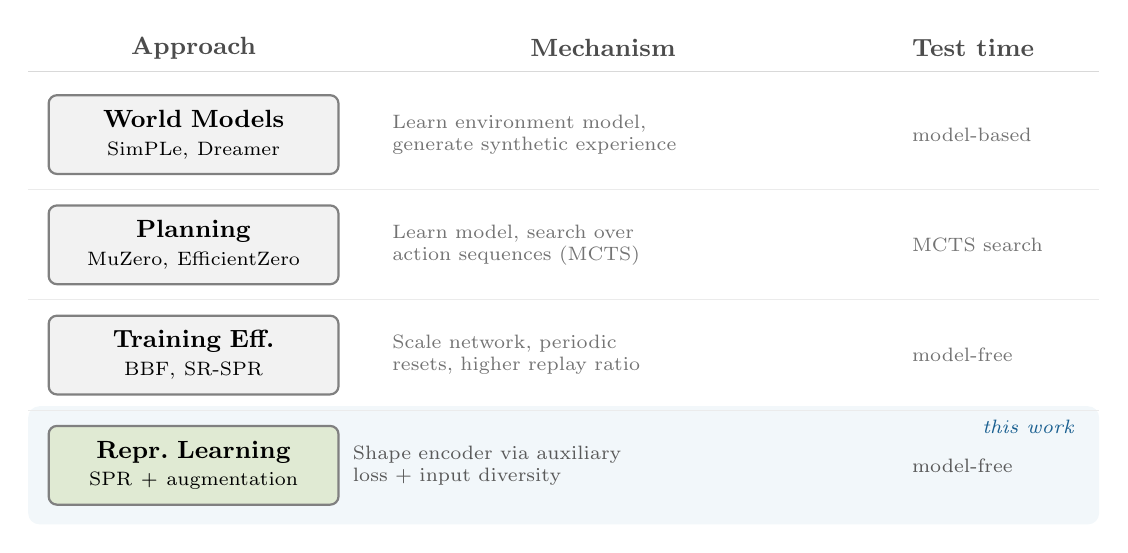
\begin{tikzpicture}[
    family/.style={draw=black!50, thick, rounded corners=3pt,
        minimum height=1.0cm, text width=3.4cm, align=center,
        font=\small, inner sep=4pt, fill=#1},
    mech/.style={font=\scriptsize, text=black!55, text width=3.8cm,
        align=left},
    ttime/.style={font=\scriptsize, text=black!55, anchor=west},
    heading/.style={font=\small\bfseries, text=black!70},
]

% === Column positions ===
\def\colA{0.3}     % Approach
\def\colB{5.5}     % Mechanism
\def\colC{10.2}    % Test time

% === Column headers ===
\node[heading] at (\colA, 0) {Approach};
\node[heading] at (\colB, 0) {Mechanism};
\node[heading] at (\colC, 0) {Test time};

% Divider line
\draw[black!15] (-1.8, -0.3) -- (11.8, -0.3);

% === Row 1: World Models ===
\def\rowA{-1.1}
\node[family=black!5] at (\colA, \rowA)
    {\textbf{World Models}\\[-1pt]
     {\scriptsize SimPLe, Dreamer}};
\node[mech, anchor=west] at (2.7, \rowA)
    {Learn environment model,\\
     generate synthetic experience};
\node[ttime] at (9.3, \rowA) {model-based};

% === Row 2: Planning ===
\def\rowB{-2.5}
\node[family=black!5] at (\colA, \rowB)
    {\textbf{Planning}\\[-1pt]
     {\scriptsize MuZero, EfficientZero}};
\node[mech, anchor=west] at (2.7, \rowB)
    {Learn model, search over\\
     action sequences (MCTS)};
\node[ttime] at (9.3, \rowB) {MCTS search};

% Row divider
\draw[black!8] (-1.8, -1.8) -- (11.8, -1.8);

% === Row 3: Training Efficiency ===
\def\rowC{-3.9}
\node[family=black!5] at (\colA, \rowC)
    {\textbf{Training Eff.}\\[-1pt]
     {\scriptsize BBF, SR-SPR}};
\node[mech, anchor=west] at (2.7, \rowC)
    {Scale network, periodic\\
     resets, higher replay ratio};
\node[ttime] at (9.3, \rowC) {model-free};

% Row divider
\draw[black!8] (-1.8, -3.2) -- (11.8, -3.2);

% === Row 4: This work (highlighted) ===
\def\rowD{-5.3}
\fill[palA!6, rounded corners=4pt]
    (-1.8, -4.55) rectangle (11.8, -6.05);

\node[family=sprcomp!50] at (\colA, \rowD)
    {\textbf{Repr.\ Learning}\\[-1pt]
     {\scriptsize SPR + augmentation}};
\node[mech, anchor=west, text=black!65] at (2.2, \rowD)
    {Shape encoder via auxiliary\\
     loss + input diversity};
\node[ttime, text=black!65] at (9.3, \rowD) {model-free};

% "This work" marker
\node[font=\scriptsize\itshape, text=palA!80!black,
    anchor=north east] at (11.6, -4.6) {this work};

% Row divider
\draw[black!8] (-1.8, -4.6) -- (11.8, -4.6);

\end{tikzpicture}
\caption{Data-efficient RL approaches. Each family addresses the
  limited-data problem through a different mechanism. This work
  studies representation learning in isolation -- the only approach
  that shapes the encoder without adding test-time computation or
  model-based planning.}
\label{fig:method-landscape}
\end{figure}


\smallskip
The methods surveyed above all target data-efficient RL, but none
ask \emph{when} self-supervised representation learning works or
what determines whether the learned representations are useful. The
original SPR paper~\citep{schwarzer2021dataefficient} evaluated SPR
exclusively on Rainbow. Follow-up work -- BBF, SR-SPR -- continued
to use Rainbow or enhanced architectures as the base agent. No
published work has tested SPR on vanilla DQN, which means the field
does not know whether SPR's representation learning is
independently effective or whether it requires a capable base agent
to produce useful representations.

\smallskip
Existing evaluations also compare methods by final performance
scores -- mean return, human-normalized score, IQM -- without
examining what the learned representations actually encode. No
prior work has compared representations across different base
agents using interpretability tools such as linear probing or
latent space visualization. Such a comparison can reveal whether
SPR produces qualitatively different representations depending on
the base agent, or whether the same representations are learned
but exploited differently by the downstream Q-head.

\smallskip
This work does not aim to beat published scores on Atari-100K.
World models, planning methods, and training efficiency
improvements have all achieved results that a vanilla DQN study
cannot match. The value lies in answering a question that
performance-focused work cannot: what determines whether
self-supervised representations are useful? By isolating SPR from
its base agent, combining it with data augmentation as a second
experimental factor, and probing the learned representations across
capability levels, this work provides controlled evidence about the
interaction between representation learning and agent capability.
The following chapter describes how we implement this study: the
agents, the experimental design, and the interpretability methods
used to probe the learned representations.
